\textbf{COLUNI 2023 -- Questão 23}\par\medskip Um estudante, durante uma aula de laboratório de Ciências, usa um dispositivo óptico para fazer a leitura do roteiro de aula, conforme mostrado na figura.

% COLUNI-AUTO-FIGURES-BEGIN
\begin{figure}[htbp]
\centering
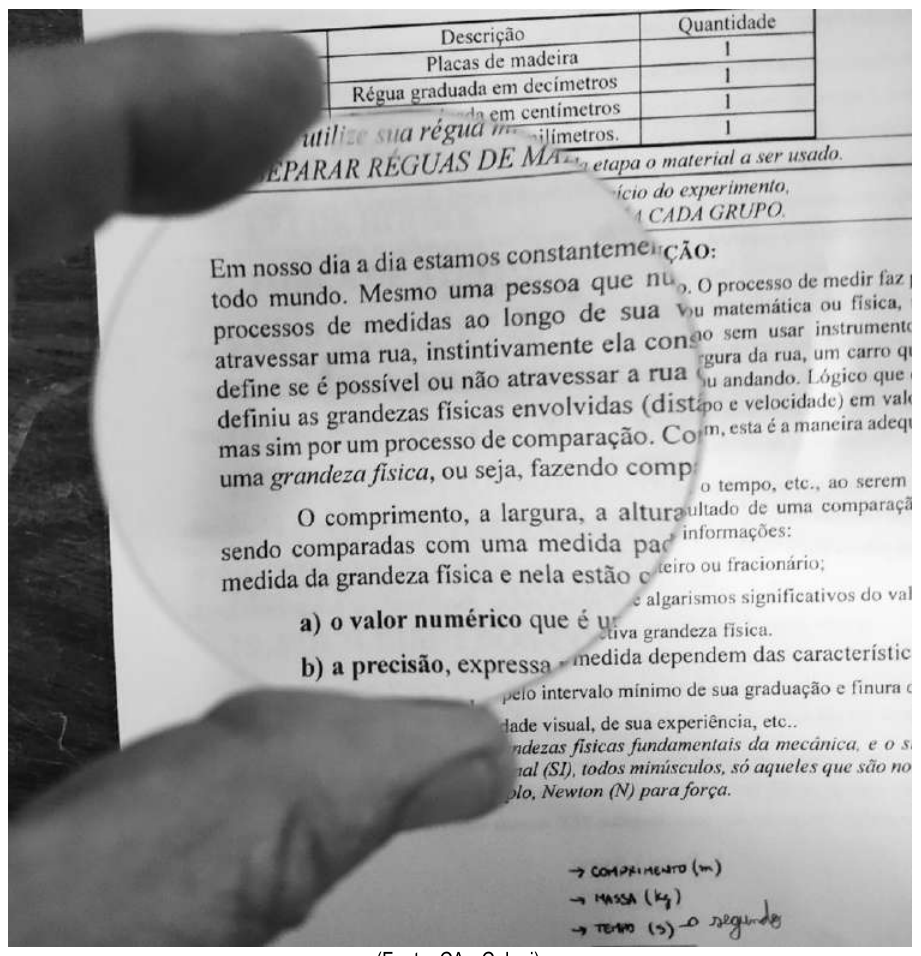
\includegraphics[width=0.95\linewidth]{static/simulados/coluni/figuras/2023/questao-23/figura-1.png}
\end{figure}
% COLUNI-AUTO-FIGURES-END
\begin{center}(Fonte: CAp-Coluni)\end{center}

Sobre o dispositivo óptico, mostrado na figura, é CORRETO afirmar:
\begin{enumerate}
\item É uma lente convergente e o fenômeno predominante é a reflexão da luz.
\item É uma lente convergente e o fenômeno predominante é a refração da luz.
\item É uma lente divergente e o fenômeno predominante é a reflexão da luz.
\item É uma lente divergente e o fenômeno predominante é a refração da luz.
\end{enumerate}
